\subsection{Technology description}

The idea consists of a welding robot, which is able to recognize a line prepared for welding. 
To be able to do this, we have to use different technology, as it is a complex case that requires a variety of components to carry out this project.

It is necessary to have a welding robot with a lot of sensors to allow the robot to be more independent. 
Standard welding robot, which can support up to 6kg with a range of 810mm (to 5 axis) would be used. 
These robots are perfect for arc welding, assembly, cleaning etc. so it is ideal to use this type of robot.

We also have to take into account all types of protection needed for the implementation of these robots, in this case the following would be used:
\begin{itemize}
\item Foundry Plus
\item Wash
\item Clean Room ISO Class 6
\end{itemize}

\begin{figure}[ht]
\centering
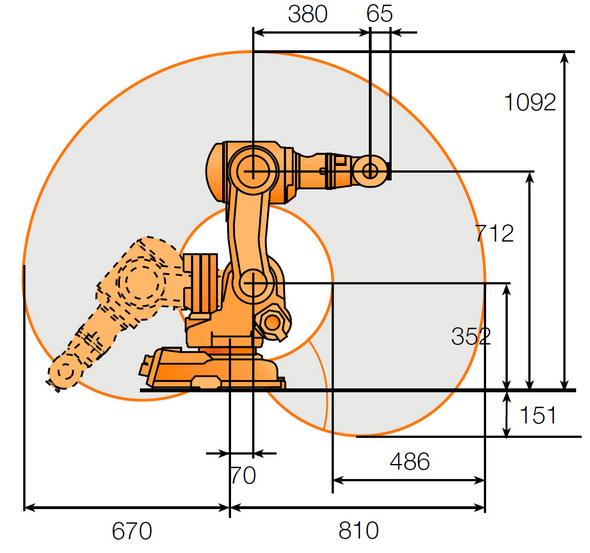
\includegraphics[width=0.3\textwidth]{./graphics/robot.png}
\caption{Possible type of robotic arm used}
\label{fig:robot}
\end{figure}

We would like the robot to be able to precisely weld holes, which can be as small as 0,1 mm. Precision of the robot is a key component for this task so we have to use a measuring tool.

The decision fell on a laser sensor capable of measuring the distance between the laser and the item prepared for welding, so knowing the position of the laser, we are able to calculate the position of the tool tip, in this case a welding pen. This will serve to correct deviations and obtain a uniform weld, because welding is performed at the same distance.

